\documentclass[a4paper]{report}

\usepackage[utf8]{inputenc}
\usepackage[english, polish]{babel}
\usepackage[T1]{fontenc}
\usepackage{indentfirst}
\usepackage[nottoc,numbib]{tocbibind}
\usepackage[font=small,labelfont=bf]{caption}
\usepackage{titlesec}
\usepackage{textcomp}
\usepackage{titling}
\usepackage{tikz}
\usetikzlibrary{decorations.markings}
\usepackage{xstring}
\let\lll\undefined
\usepackage{amssymb,amsthm,amsmath}
\usepackage{mathtools}
\mathtoolsset{showonlyrefs}
\usepackage[unicode]{hyperref}
\usepackage{booktabs}

\titleformat{\chapter}[hang]
    {\Large\fillast}
    {\oldstylenums{\thechapter} }
    {0pt}
    {\scshape\bfseries}

\titleformat{\section}[hang]
    {\large\fillast}
    {\oldstylenums{\thesection} }
    {0pt}
    {\scshape}

\titleformat{\subsection}[hang]
    {\large\fillast}
    {\oldstylenums{\thesubsection} }
    {0pt}
    {\itshape\scshape}

\theoremstyle{definition}
\newtheorem{definition}{Definicja}[chapter]    

\begin{document}
\begin{titlepage}
\begin{center}
    \LARGE
    \textbf{Jagiellonian University}\\
    Theoretical Computer Science Department

    \vspace{1.5in}
    \Large
    \textbf{Piotr Helm}

    \large
    Nr albumu: 1132708
    
    \vspace{0.5em}
    \LARGE
    \rule{\textwidth}{1pt}
    \textsc{Coreset constructions for Kmeans Problem}
    \rule{\textwidth}{1pt}

    \vspace{1em}
    \Large
    \textbf{Bachelor’s thesis}\\

    \large
    \vspace{1in}
    \hfill
    \parbox{0.8\textwidth}{
        Supervisor \\
        \textbf{dr Iwona Cieślik} \\
        Theoretical Computer Science Department\\
        of Jagiellonian University
        }

    \vfill
    \Large
    Kraków, August 2020
\end{center}
\end{titlepage}

\thispagestyle{empty}
\begin{abstract}
    W pracy przedstawimy stan wiedzy na temat budowania coresetów w kontekście problemu $k$-means.
    W szczególności omówimy techniki konstrukcji coresetów takie jak geometryczna dekompozycja oraz losowe próbkowanie z \cite{DBLP:journals/ki/MunteanuS18}.
    Celem pracy jest przedstawienie wyników teoretycznych oraz implementacja technik budowania coresetów \cite{DBLP:journals/ki/MunteanuS18} \cite{bachem2017scalable}.
\end{abstract}

\chapter{Introduction}

TBA
\chapter{Notacja i niezbędne definicje}\label{preliminaries}

W tej pracy przyjmujemy, że działamy w przestrzeni euklidesowej w skończonym wymiarze $d > 0$.

\begin{definition}
    \emph{Norma typu $l_{2}$} dla $x \in \mathbb{R}^d$ to:
    \begin{equation}
        ||x||_{2} = ||x|| = \sqrt{ \sum_{i = 1}^{d} x_{i}^{2} }
    \end{equation}
\end{definition}

\noindent
Załóżmy, że mamy dany konkretny problem optymalizacyjny. 
Niech $F(x)$ oznacza zbiór dopuszczalnych rozwiązań tego problemu dla danych wejściowych $x$. 
Niech $c(y) \leq 0$ gdzie $ y\in F(x)$ będzie funkcją kosztu rozwiązania dla tego problemu.
Oznaczmy przez $c_{opt}(x)$ koszt rozwiązania optymalnego dla danych $x$.

\begin{definition}
    \emph{$\epsilon$-aproksymacja.} 
    Algorytm A nazywamy $\epsilon$-aproksymacyjnym, jeżeli dla dowolnych poprawnych danych wejściowych $x$, $A(x) \in F(x)$ oraz:
    \begin{equation}
        \frac{|c(A(x)) - C_{opt}(x) |}{ \max\{c(A(x)),C_{opt}(x) \} } \leq \epsilon
    \end{equation}
    gdzie $\epsilon \in [0,1]$ nazywamy \textit{błędem aproksymacji}.
\end{definition}

\begin{definition}
    \emph{Centroid} dla skończonego zbioru punktów $x_{1}, \dots, x_{k} \in \mathbb{R}^{d}$ to:
    \begin{equation}
        C = \frac{x_{1} + \dots + x_{k}}{k}
    \end{equation}
    gdzie punkt $C$ minimalizuje sumę kwardatów odległości pomiedzy nim samym a punktami $x_{1}, \dots, x_{k}$.
\end{definition}

\noindent
Często utożamaiamy centroid z punktami dla których jest on centroidem.
W takiej sytuacji użyjemy stwierdzenia \textit{środek centroidu} do nazwania zdefiniowanego w 2.3 faktycznego centroidu.

\begin{definition}
    \emph{Klaster} to skończony zbioru punktów $x_{1}, \dots, x_{k} \in \mathbb{R}^{d}$, które łaczy wspólna cech.
    W naszym kontekście wspólną cechą bedzie przyporządkowanie do tego samego centroidu.
\end{definition}

\section{K-means}

Zacznijmy od zdefiniowania problemu dla którego będziemy analizować konstrukcje coresetów.

\begin{definition}
    \emph{Problem K-means.} Niech $X$ to skończony zbiór punktów z $\mathbb{R}^{d}$. 
    Dla danego $X$ chcemy znalźć zbiór $k \in \mathbb{N}$ punktów $Q \subset \mathbb{R}^{d}$, który minimalizuje funkcję $\phi_{X}(Q)$ zdefiniowaną następująco:
    \begin{equation}
        \phi_{X}(Q) = \sum_{x \in X} d(x, Q)^{2} = \sum_{x \in X} \min_{q \in Q} || x - q ||^{2} 
    \end{equation}
\end{definition}

\noindent
Definicja 2.2 zakłada, że działamy w przestrzeni euklidesowej.
Uogólnioną wersję można zdefiniować analogicznie, zamieniając $d$ na odpowiednią funkcję miary w danej przestrzeni.

\begin{definition}
    \emph{Problem K-means - wersja ważona.} Niech $C$ to skończony zbiór punktów z $\mathbb{R}^{d}$ oraz niech $w$ będzie funkcją $C \rightarrow \mathbb{R}_{\ge0}$. 
    Dla danego $C$ oraz funkcji $w$ chcemy znaleźć zbiór $k \in \mathbb{N}$ punktów $Q$, który minimalizuje funkcję $\phi_{C}(Q)$ zdefiniowaną następująco:
    \begin{equation}
        \phi_{C}(Q) = \sum_{c \in C} w(c) d(c, Q)^{2}
    \end{equation}
\end{definition}

\noindent
Ewaluację funkcji $\phi$ dla optymalnego rozwiązania oznaczamy $\phi_{opt}^{k}(X)$ lub $OPT$.
W pracy często będziemy korzystać ze stwierdzenia \textit{optymalne rozwiązanie}, które oznacza $k$ elementowy zbiór dla którego wartość funkcji $\phi$ jest zminimalizowana. 
Funkcję $\phi$ w literaturze nazywamy błędem kwantyzacji.

\section{Coreset}

To jak definujemy coreset ściśle zależy od problemu, który optymalizujemy.
Zacznijmy od podstawowej definicji coresetu dla problemu K-means.

\begin{definition}
    \emph{Coreset.} Niech $X$ to skończony zbiór punktów z $\mathbb{R}^{d}$ oraz niech $Q$ to dowolny podzbiór $X$ rozmiaru co najwyżej $k$. 
    Skończony zbiór $C \subset R^{d}$ nazywamy $(\epsilon, k)$ coresetem, gdzie $\epsilon \in (0, 1)$, jeżeli zachodzi:
    \begin{equation}
        |\phi_{X}(Q) - \phi_{C}(Q)| \leq \epsilon\phi_{X}(Q)
    \end{equation}
\end{definition}

\noindent
Zauważmy, że taka definicja daje nam bardzo moce gwarancje teoretyczne.
Wartość funkcji $\phi_{C}(Q)$ aproksymuje $\phi_{X}(Q)$ z błędem $(1+\epsilon)$ dla dowolnego zbioru $k$ kandydatów na rozwiązanie $Q$.
Jest to na tyle istotne, że w literaturze odróżnimy taką wersję nazywając ją \textit{strong coresetem}.

\begin{definition}
    \emph{Coreset - weak.} Niech $X$ to zbiór punktów z $\mathbb{R}^{d}$ oraz $\epsilon \in (0, 1)$.
    Słabym coresetem nazywamy skończony zbiór $C \subset \mathbb{R}^d$ dla którego zachodzi:
    \begin{equation}
        |\phi_{X}(Q) - \phi_{C}(Q)| \leq \epsilon\phi_{X}(Q)
    \end{equation}
\end{definition}

%dyskretna/ciągła 
\chapter{Lightweight Coreset}

Budowa coresetów w kontekście problemu \textit{k-means} ma bardzo długo historię.
Za przełomową pracę uznaje się \cite{Matousek99onapproximate}, która jako 
pierwsza przedstawiła wielomianowy schemat aproksymacji o złożoności $O(n\epsilon^{-2k^2d}\log^kn)$ budujący coreset dla problemu $k$-means.
\\~\\
Wyróżnia się trzy techniki budowania coresetów:
\begin{itemize}
    \item Geometryczna dekompozycja problemu.
    \item Losowe próbkowanie zbioru.
    \item Zawansowane metody algebraiczne.
\end{itemize}
Pierwsza i trzecia technika cechuje się mocnymi gwarancjami teoretycznymi.
Niestety większość rozwiązań jest mało praktyczna i kosztowna czasowo.
Losowe próbkowanie w praktyce daje bardzo przyzwoite wyniki jednak bardzo często nie daje nam żadnej gwarancji odnośnie optymalności rozwiązania.
Autorzy pracy \cite{bachem2017scalable} zaproponowali rozwiązanie o nazwie \textit{lightweight coreset}, które w swoich założeniach ma łączyć:
\begin{itemize}
    \item Prostą implementacje.
    \item Gwarancje teoretyczne.
    \item Szybkie działanie oparte na próbkowaniu zbioru danych.
\end{itemize}
\section{Lightweight coreset}

Zacznijmy od wprowadzenia definicji \textit{lightweight coresetu}.
\begin{definition}
    \emph{Lightweight coreset dla problemu K-means.} Niech $\epsilon > 0$ oraz $k \in \mathbb{N}$.
    Niech $X$ bedzie $n$ elementowym zbiórem punktów z $\mathbb{R}^{d}$ wraz ze średnią $\mu(X) = \frac{1}{n}\sum_{i=1}^{n} x_{i}$.
    Zbiór $C \subset \mathbb{R}^d$ jest $(\epsilon, k)$ lightweight coresetem jeżeli dla dowolnego zbioru $Q \subset \mathbb{R}^{d}$ o mocy co najwyżej $k$ zachodzi:
    \begin{equation}
        |\phi_{X}(Q) - \phi_{C}(Q)| \leq \frac{\epsilon}{2}\phi_{X}(Q) + \frac{\epsilon}{2}\phi_{X}(\mu(X))
    \end{equation}
\end{definition}

\noindent
Jak możemy zauważyć definicja (3.1) trochę się różni od (2.8).
Notacje \textit{lightweight} coresetu możemy interpretować jako relaksację gwarancji teoretycznych zdefiniowanych w (2.8).
Wprowadza ona oprócz błędu multiplikatywnego, błąd addytywny.
Nieformalnie, składnik $\frac{\epsilon}{2}\phi_{X}(Q)$ pozwala na odpowiednie skalowanie błędu aproksymacji dla funkcji $\phi$, jest on tożsamy z błędem aproksymacji coresetu zdefiniowanego w 2.8.
Druga część $\frac{\epsilon}{2}\phi_{X}(\mu(X))$ odpowiada za skalowalność rozwiązania zgodnie ze zmianą wariancji na danych.
Przez skalowalność rozumiemy zmianę rozmiaru danych, mocy zbiorów.

Głowną motywacją stojącą za konstrukcjami coresetów jest to, żeby rozwiązanie obliczone na tym zbiorze było konkurencyjne z rozwiazaniem optymalnym dla całego zbioru danych.
Dlatego w konkeście \textit{lightweight} udowodnimy następujące twierdzenie.

\begin{thm}{\cite{bachem2017scalable}}
    Niech $\epsilon \in (0, 1]$. Niech $X$ będzie skończonym zbiorem danych z $\mathbb{R}^d$ oraz niech $C$ będzie $(\epsilon, k)$ lightweight coresetem dla $X$.
    Optymalne rozwiązanie problemu K-means dla $X$ oznaczamy $Q_{X}^{*}$.
    Optymalne rozwiązanie problemu K-means dla $C$ oznaczamy $Q_{C}^{*}$.
    Dla takich założeń zachodzi:
    \begin{equation}
        \phi_{X}(Q_{C}^{*}) \leq \phi_{X}(Q_{X}^{*}) + 4\epsilon\phi_{X}(\mu(X))
    \end{equation}
\end{thm}

\begin{proof}
    Zgodnie z własnością lightweight coresetu otrzymujemy:
    \begin{equation}
        \phi_{C}(Q_{X}^{*})  \leq (1+\frac{\epsilon}{2})\phi_{X}(Q_{X}^{*}) + \frac{\epsilon}{2}\phi_{X}(\mu(X))
    \end{equation}
    oraz
    \begin{equation}
        \phi_{C}(Q_{C}^{*})  \geq (1-\frac{\epsilon}{2})\phi_{X}(Q_{C}^{*}) - \frac{\epsilon}{2}\phi_{X}(\mu(X))
    \end{equation}
    Wiemy z definicji, że $\phi_{C}(Q_{C}^{*}) \leq  \phi_{C}(Q_{X}^{*})$ oraz $1 - \frac{\epsilon}{2} \geq \frac{1}{2}$.
    A więc:
    \begin{equation}
        \phi_{X}(Q_{C}^{*}) \leq \frac{1+\frac{\epsilon}{2}}{1-\frac{\epsilon}{2}}\phi_{X}(Q_{X}^{*}) + \frac{\epsilon}{1-\frac{\epsilon}{2}}\phi_{X}(\mu(X))
    \end{equation}
    \begin{equation}
        \leq (1+2\epsilon)\phi_{X}(Q_{X}^{*}) + 2\epsilon\phi_{X}(\mu(X))
    \end{equation}
    Zauważając, że:
    \begin{equation}
        \phi_{X}(Q_{X}^{*}) \leq \phi_{X}(\mu(X))
    \end{equation}
    dowodzimy tezę twierdzenia.
\end{proof}

\noindent
Twierdzenie 1 dowodzi, że kiedy wartość $\epsilon$ maleje koszt optymalnego rozwiązania otrzymanego na zbiorze $C$ zbiega do kosztu rozwiązania otrzymanego na całym zbiorze danych.
\section{Konstrukcja}

Konstrukcja oparta jest na próbkowaniu z uwzględnieniem ważności danego punktu.
Niech $q(x)$ będzie dowolnym rozkładem prawdopodobieństwa na zbiorze $X$ oraz niech $Q \subset R^{d}$ będzie dowolnym potencjalnym zbiorem rozwiązań mocy $k$. 
Wtedy funkcję $\phi$ możemy zapisać jako:

\begin{equation}
    \phi_{X}(Q) = \sum_{x \in X} q(x) \frac{d(x, Q)^{2}}{q(x)}
\end{equation}

\noindent
Wynika z tego, że funkcja $\phi$ może być aproksymowana poprzez wylosowanie $m$ punktów z $X$ korzystając z $q(x)$ i przypisując im wagi odwrotnie proporcjonalne do $q(x)$.
Dla dowolnej liczby próbek $m$ oraz dla dowolnego rozkładu $q(x)$ możemy otrzymać sprawiedliwy (unbiased) estymator dla funkcji $\phi$.
Niestety, nie jest to wystarczające aby spełnić definicję (3.1).
W szczególności musimy zagwarantować, jednostajność wyboru dowolnego zbioru $k$ punktu $Q$ z odpowiednim prawdopodobieństwem $1 - \delta$.
Funkcja $q(x)$ może mieć wiele form, autorzy rekomendują postać:
\begin{equation}
    q(x) = \frac{1}{2}\frac{1}{|X|} + \frac{1}{2}\frac{d(x, \mu)^2}{\sum_{x^{'} \in X}d(x^{'}, \mu)^2}
\end{equation}

\begin{algorithm}
    \caption{}
\begin{algorithmic}
    \Procedure{Lightweight}{} \Comment{Require: Set of data points X, coreset size m}
        \State $\mu \leftarrow$ mean of $X$
        \For{$x \in X$}                    
            \State $q(x) = \frac{1}{2}\frac{1}{|X|} + \frac{1}{2}\frac{d(x, \mu)^2}{\sum_{x^{'} \in X}d(x^{'}, \mu)^2}$
        \EndFor
        \State $C \leftarrow$ sample $m$ weighted points from $X$ where each point $x$ has weight $\frac{1}{mq(x)}$ and is sampled with probability $q(x)$
    \EndProcedure
    \Return lightweight coreset C
\end{algorithmic}
\end{algorithm}

\noindent
Pierwszy składnik rozkładu $q(x)$ to rozkład jednostajny, który zapewnia, że każdy punkt jest wylosowany z niezerowym prawdopodobieństwem.
Drugi składnik uwzględnia kwadrat odległości punktu od średniej $\mu(X)$ dla całego zbioru.
Intuicyjnie, punkty, które są daleko od średniej $\mu(X)$ mogą mieć istotny wpływ na wartość funkcji $\phi$.
Musimy więc zapewnić, odpowiednią częstotliwość wyboru takich punktów. 
Jak pokazuje pseudokod, implementacja takiej konstrukcji jest całkiem prosta.
Zauważmy, że jest ona też bardzo praktyczna.
Algorytm przechodzi przez zbiór danych jedynie dwukrotnie, a jego złożoność to $O(nd)$.
Nie mamy zależności od $k$ co jest kluczowe w konkeście praktyczności takiego rozwiązania.
\section{Analiza}

W tej części udowodnimy, że zaproponowany w poprzedniej części algorytm oblicza lightweight coreset dla odpowiedniego $m$.

\begin{thm}{\cite{bachem2017scalable}}
    Niech $\epsilon > 0$, $\delta > 0$ oraz $k \in \mathbb{N}$. 
    Niech $X$ to skończony zbiór punktów z $\mathbb{R}^{d}$ oraz $C \subset X$ to zbiór zwracany przez algorytm dla:
    \begin{equation}
        m \geq c\frac{dk \log{k} + \log{\frac{1}{\delta}}}{\epsilon^2} 
    \end{equation}
    gdzie $c$ to stała. 
    Wtedy z prawdopodobieństwem co najmniej $1-\delta$ zbiór $C$ jest $(\epsilon, k)$ lightweight coresetem dla $X$.
\end{thm}

\begin{proof}

\noindent
Zacznę od ograniczenia ważności dla każdego punktu $x \in X$. 
W tym celu definiuje funkcję:

\begin{equation}
    f(Q) = \frac{1}{2|X|}\phi_{X}(Q) + \frac{1}{2|X|}\phi_{X}(\mu(X))
\end{equation}

\noindent
gdzie $\mu(X)$ to średnia zbioru $X$ oraz dowodzę następujący lemat. 

\begin{lemma}{\cite{bachem2017scalable}}
    Niech $X$ to skończony zbiór punktów z $\mathbb{R}^{d}$ wraz ze średnią $\mu(X)$. 
    Dla każdego $x \in X$ oraz $Q \subset \mathbb{R}^{d}$ zachodzi:
    \begin{equation}
        \frac{d(x, Q)^2}{f(Q)} \leq \frac{16d(x, \mu(X))^2}{\frac{1}{|X|}\sum_{x^{'} \in X}d(x^{'}, \mu(X))^2} + 16
    \end{equation}
\end{lemma}

\begin{proof}
    \noindent
    Z nierówności trójkąta oraz z faktu, że $(|a| + |b|)^2 = 2a^2 + 2b^2$, otrzymujemy
    \begin{equation}
        d(\mu(X), Q)^2 \leq 2d(x, \mu(X))^2 + 2d(x, Q)
    \end{equation}
    
    \noindent
    Uśrednienie dla wszystkich $x \in X$, implikuje:

    \begin{equation}
        d(\mu(X), Q)^2 \leq \frac{2}{|X|} \sum_{x \in X} d(x, \mu(X))^2 + \frac{2}{|X|} \sum_{x \in X} d(x, Q)
    \end{equation}
    \begin{equation}
       = \frac{2}{|X|} \phi_{X}(\mu(X))+ \frac{2}{|X|} \phi_{X}(Q)
    \end{equation}

    \noindent
    To implikuje, że dla każdego $x \in X$ oraz $Q \subset \mathbb{R^d}$ zachodzi:

    \begin{equation}
        d(x, Q)^2 \leq 2d(x, \mu(X))^2 + 2d(\mu(X), Q)
    \end{equation}

    \begin{equation}
       \leq 2d(x, \mu(x))^2 +  \frac{4}{|X|} \phi_{X}(\mu(X))+ \frac{4}{|X|} \phi_{X}(Q)
    \end{equation}

    \noindent
    Dzieląc powyższą nierówność przez wyżej zdefiniowaną funkcję $f(Q)$ dostajemy:

    \begin{equation}
        \frac{d(x, Q)^2}{f(Q)} \leq \frac{2d(x, \mu(x))^2 +  \frac{4}{|X|} \phi_{X}(\mu(X))+ \frac{4}{|X|} \phi_{X}(Q)}{\frac{1}{2|X|}\phi_{X}(Q) + \frac{1}{2|X|}\phi_{X}(\mu(X))}
    \end{equation}

    \begin{equation}
        \leq \frac{2d(x, \mu(x))^2 +  \frac{4}{|X|} \phi_{X}(\mu(X))}{\frac{1}{2|X|}\phi_{X}(\mu(X))} + \frac{\frac{4}{|X|} \phi_{X}(Q)}{\frac{1}{2|X|}\phi_{X}(Q)}
    \end{equation}

    \begin{equation}
        \leq \frac{16d(x, \mu(X))^2}{\frac{1}{|X|}\sum_{x^{'} \in X}d(x^{'}, \mu(X))^2} + 16
    \end{equation}

    \noindent
    co kończy dowód lematu.
\end{proof}

\noindent
Powyższy lemat implikuje, że stosunek pomiędzy kosztem kontrybucji $d(x, Q)^2$ jednego punku $x \in X$ a $f(Q)$ jest ograniczony dla każdego $Q \subset X$ przez:

\begin{equation}
    s(x) = \frac{16d(x, \mu(X))^2}{\frac{1}{|X|}\sum_{x^{'} \in X}d(x^{'}, \mu(X))^2} + 16    
\end{equation}

\noindent
Zdefinuje $S = \frac{1}{|X|} \sum_{x \in X}s(x)$ zauważając, że 
\begin{equation}
    S =  \frac{1}{|X|}  \sum_{x \in X}s(x)  =  \frac{1}{|X|} \sum_{x \in X} \Big( \frac{16d(x, \mu(X))^2}{\frac{1}{|X|}\sum_{x^{'} \in X}d(x^{'}, \mu(X))^2} + 16 \Big)
\end{equation}
\begin{equation}
    =  \frac{1}{|X|} \sum_{x \in X} \Big( \frac{16d(x, \mu(X))^2}{\frac{1}{|X|}\sum_{x^{'} \in X}d(x^{'}, \mu(X))^2} \Big) + \frac{1}{|X|} \sum_{x \in X} 16 
\end{equation}
\begin{equation}
    = \frac{16  \sum_{x \in X}  d(x, \mu(X))^2}{\sum_{x^{'} \in X}d(x^{'}, \mu(X))^2} + 16 = 32
\end{equation}
dla każdego zbioru $X$.
Dzięki temu mogę zapisać rozkład $q$ jako:

\begin{equation}
    q(x) = \frac{1}{2}\frac{1}{|X|} + \frac{1}{2}\frac{d(x, \mu(X))^2}{\sum_{x^{'} \in X}d(x^{'}, \mu(X))^2} = \frac{s(x)}{S|X|}
\end{equation}

\noindent
dla każdego $x \in X$. Rozpatruję funkcję:

\begin{equation}
    g_{Q}(x) = \frac{d(x, Q)^2}{f(Q)s(x)}
\end{equation}

\noindent
dla każdego $x \in X$ oraz $Q \subset \mathbb{R^d}$.
Zauważmy, że dla dowolnego zbioru  $Q \subset \mathbb{R}^{d}$ zachodzi:

\begin{equation}
    \phi_{X}(Q) = \sum_{x \in X} d(x, Q)^2 = S|X|f(Q) \sum_{x \in X} \frac{s(x)}{S|X|} \frac{d(x, Q)^2}{f(Q)s(x)}
\end{equation}

\begin{equation}
    =  S|X|f(Q) \sum_{x \in X} q(x) g_{Q}(x)
\end{equation}

\noindent
Następnie podstawiamy z definicji wartości oczekiwanej:

\begin{equation}
    \mathbb{E}_q[g_{Q}(x)] = \sum _{x \in X} q(x) g_{Q}(x)
\end{equation}

\noindent
dzięki temu przekształcamy ostatnie równanie:

\begin{equation}
    \phi_{X}(Q) = S|X|f(Q)\mathbb{E}_q[g_{Q}(x)]
\end{equation}

\noindent
Następnym krokiem jest ograniczenie wartości $\mathbb{E}_q[g_{Q}(x)]$.
Autorzy \cite{bachem2017scalable} nie dowodzą wprost tego ograniczenia, powołując się na inne prace.
Dowód jest bardzo skompilowany i wykracza tematyką istotnie poza ramy tej pracy więc go pomijamy.
Korzystam z finalnego ograniczenia:

\begin{equation}
    |\mathbb{E}_q[g_{Q}(x)] - \frac{1}{|C|} \sum_{x \in X}g_{X}(x)| \leq \frac{\epsilon}{32}
\end{equation}

\noindent
Powyższe ograniczenie jest prawdziwe z prawdopodobieństwem $1 - \delta$ dla dowolnego $Q \subset \mathbb{R}^{d}$ o rozmiarze nie większym niż $k$.
Mnożąc obie strony nierówności przez $32|X|f(Q)$ otrzymujemy:

\begin{equation}
    |32|X|f(Q)\mathbb{E}_q[g_{Q}(x)] - \frac{32|X|f(Q)}{|C|} \sum_{x \in X}g_{X}(x)| \leq \epsilon|X|f(Q)
\end{equation}

\noindent
Niech $(C, u)$ będzie ważonym zbiorem, gdzie dla każdego $x \in C$ definujemy funkcję $u(x) = \frac{1}{|C|q(x)}$.
Wynika z tego, że:

\begin{equation}
    \frac{32|X|f(Q)}{|C|} \sum_{x \in X}g_{X}(x) = \sum \frac{1}{|C|q(x)} d(x, Q)^2
\end{equation}

\begin{equation}
    = \sum u(x) d(x, Q)^2 = \phi_{C}(Q)
\end{equation}

\noindent
A więc otrzymujemy:

\begin{equation}
    |32|X|f(Q)\mathbb{E}_q[g_{Q}(x)] - \phi_{C}(Q)| \leq \epsilon|X|f(Q)
\end{equation}

\begin{equation}
    |\phi_{Q}(Q) - \phi_{C}(Q)| \leq \frac{\epsilon}{2}\phi_{X}(Q) + \frac{\epsilon}{2}\phi_{X}(\mu(X))
\end{equation}

\noindent
co kończy dowód twierdzenia 3.2.

\end{proof}
\chapter{Geometryczna Dekompozycja}\label{geo}
W tej części pracy przedstawimy konstrukcję budowy coresetu bazującą na geometrycznej dekompozycji problemu.
Punktem wyjścia były badania \cite{DBLP:journals/ki/MunteanuS18}, na których bazuje opisany w podrozdziale 4.4 algorytm.
Zgodnie z nimi budowa coresetu w kontekście problemu K-means to wieloetapowy proces, który jest sekwencją algorytmów z prac: \cite{Gonzalez1985ClusteringTM} \cite{10.1145/1007352.1007400} \cite{Arya2004LocalSH} \cite{DBLP:journals/ki/MunteanuS18}.
W rozdziale przyjmujemy następujący porządek analizy konstrukcji:
\begin{itemize}
    \item W sekcjach 4.1, 4.2, 4.3 opiszemy konstrukcje pomocnicze pochodzące z prac: \cite{Gonzalez1985ClusteringTM}, \cite{10.1145/1007352.1007400}, \cite{Arya2004LocalSH}.
    \item W sekcji 4.4 opiszemy właściwy algorytm z pracy \cite{DBLP:journals/ki/MunteanuS18}.
\end{itemize}

\section{Algorytm Gonzalez'a}

Pierwszy algorytm z którego opiszę to \textit{Farthest point algorithm} z pracy \cite{Gonzalez1985ClusteringTM}.
Jest to pierwszy algorytm aproksymacyjny rozwiązująych problem k-centrów z błędem nie większem niż $2$\textit{OPT}, gdzie \textit{OPT} to optymalne rozwiązanie.
Jego złożoność to $O(nk)$, gdzie $n$ to liczba punktów. 
\\~\\
Niech $S$ to bedzie zbiór który chcemy sklastrować oraz niech $T$ będzie podzbiorem $S$.
Zakładamy, że $|S| > k$ ponieważ w przeciwnym przypadku problem jest trywialnie rozwiązywalny.
Zbiór $T$ nazywamy $(k+1)$ kliką wysokości $h$ jeżeli moc zbioru $T$ jest równa $k+1$ oraz odległość pomiędzy parą dwóch rożnych punktów jest równa co najmniej $h$. 
Niech $OPT(S)$ oznacza optymalne rozwiązanie problemu k-centrów dla zbioru $S$.
Udowodnię teraz następujący lemat, którego dowód jest opisem \textit{Farthest point algorithm}.

\begin{lemma}
    Jeżeli w zbiorze $S$ istnieje $(k+1)$ klika wysokości $h$, to $OPT(S) \geq h$.
\end{lemma}

\begin{proof}
    
\end{proof}

\begin{algorithm}
    \caption{}
\begin{algorithmic}
    \State For each point not in $T$, the algorithm keeps $neighbor(p)$, the nearest point in $T$, and $dist(p)$, the distance from $p$ to $neighbor(p)$.
    \Procedure{Farthest point algorithm}{}
        \State $T \leftarrow \emptyset$
        \State $dist(p) \leftarrow \inf$ for all $p \in S$
        \While{$|T| \leq k$}                    
            \State $D \leftarrow max\{dist(p) | p \in S-T\}$
            \State choose $p^{'}$ from $S-T$ such $dist(p^{'}) = D$
            \State add $p^{'}$ to T
            \State update $neighbor(p)$ and $dist(p)$ for all $p \in S-T$
        \EndWhile
    \EndProcedure
    \Return $T$
\end{algorithmic}
\end{algorithm}
\section{Konstrukcja kraty wykładniczej}

W tym podrozdziale omówimy część pracy \cite{10.1145/1007352.1007400}.
Tematem pracy są konstrukcje algorytmów dla problemów $k$-means oraz $k$-median.
W kontekście problemu $k$-means autorzy zaproponowali algorytm rozwiązujący problem $k$-means bazujący na budowie coresetu, który uzyskuje lepszą złożoność od \cite{Matousek99onapproximate}.
Matoušek w swojej pracy przedstawił wielomianowy schemat aproksymacji, którego złożoność to $O(n\epsilon^{-2k^2d}\log^kn)$.
Autorzy \cite{10.1145/1007352.1007400} poprawili tą złożoność uzyskując $O(n+k^{k+2}\epsilon^{-(2d+1)k}\log^{k+1}n \log^k\frac{1}{\epsilon})$.
Schemat konstrukcji jest następujący:
\begin{itemize}
    \item Obliczmy szybką ale niedokładną aproksymację dla problemu $k$-means z pewną dużą wartością $k$.
    \item Obliczoną aproksymację przekształcamy w $(\epsilon, k)$ coreset używając kraty wykładniczej.
\end{itemize}


\subsection{Szybka aproksymacja dla problemu K-means.}
\noindent
Zacznijmy od pierwszej części.
Dokładniej, udowodnimy następujące twierdzenie.

\begin{thm}{\cite{10.1145/1007352.1007400}}
    Dla danego zbioru $n$ punktów $P \subset \mathbb{R}^d$ oraz parametru $k \in \mathbb{N}$ możemy 
    obliczyć zbiór $X$ o mocy $O(k \log^{3}n)$, dla którego 
    \begin{equation}
        \phi_{P}(X) \leq 20 \phi_{opt}^{k}(P)
    \end{equation}
    Czas działania algorytmu to $O(n)$ dla $k = O(n^{\frac{1}{4}})$ oraz $O(n \log (k \log n))$ w przeciwnym przypadku.
\end{thm}

\noindent
Niech $P \subset \mathbb{R}^{d}$ będzie danym na wejściu zbiórem $n$ punktów.
Chcemy szybko obliczyć aproksymację dla problemu $k$-means na tym zbiorze, gdzie rozmiar wynikowego zbioru punktów będzie rzędu $O(k \log^{3}n)$.

\begin{definition}
    \emph{Złe/dobre punkty.} Dla zbioru punktów $X$, punkt $p \in P$ nazywamy \textit{złym} jeżeli
    \begin{equation}
        d(p, X) \geq 2d(p, C_{opt})
    \end{equation}
    gdzie $C_{opt}$ jest zbiórem punktów realizującym $\phi_{opt}^{k}(P)$.
    Punkt jest \textit{dobry} jeżeli nie jest zły.
\end{definition}

\noindent
Na początku opiszemy procedurę, która dla danego $P$, wyznacza zbiór punktów $X$ o mocy rzędu $O(k \log^{2}n)$ oraz zbiór $P^{'} \subset P$.
Zbiór $P^{'}$ będzie zawierać \textit{dobre} punkty dla zbioru $X$.
\\~\\
Konstrukcję zbioru $X$ zaczynamy od obliczenia 2-aproksymacji problemu k-centrów dla zbioru $P$.
Niech obliczony zbiór centrów to $V$.
Taką aproksymację dla $k = O(n^{\frac{1}{4}})$ możemy obliczyć w czasie $O(n)$ oraz dla $k = \Omega(n^{\frac{1}{4}})$ w czasie $O(n \log k)$ \cite{10.1145/62212.62255}.
Są to wyniki teoretyczne, które zakładamy na potrzebę analizy.
W podrozdziale 4.1 przedstawiliśmy algorytm aproksymacyjny rozwiązujący ten problem w czasie $O(nk)$ dla dowolnego $k$.
Algorytmy o lepszej złożoności są w istotny sposób bardziej skomplikowane, dlatego w naszej implementacji zastosowaliśmy algorytm Gonzaleza.
Niech $L$ będzie promieniem takiej aproksymacji, czyli największą odległością pomiędzy punktem $v \in V$ a punktem $p \in P-V$.
Ponieważ algorytm z pracy \cite{10.1145/62212.62255} bazuje na algorytmie przedstawionym w podrozdziale 4.1 z pracy \cite{Gonzalez1985ClusteringTM} to dystans pomiędzy dowolną parą punktów z $V$ wynosi co najmniej $L$.
To implikuje następujące ograniczenia:
\begin{equation}
    \Big( \frac{L}{2 } \Big)^2 \leq \phi_{opt}^{k}(V) \leq \phi_{opt}^{k}(P) \leq nL^{2}
\end{equation}
Dolne ograniczenie argumentujemy tym, że możemy ograniczyć $\phi_{opt}^{k}(V)$ przez $d(v_{1}, v_{2})^2$, gdzie $v_{1}, v_{2} \in V$.
Górne ograniczenie wynika z faktu, że promień aproksymacji jest równy $L$, więc dla $n$ elementowego zbioru $P$ wartość funkcji $\phi_{opt}^{k}(P)$ nie może być większa niż $nL^2$.
\\~\\
Następnym krokiem konstrukcji jest wylosowanie $\rho = \gamma k \log^{2} n$ punktów ze zbioru $P$, gdzie $\gamma$ jest stałą, która wynika z analizy, którą zaraz przeprowadzimy.
Niech $Y$ będzie zbiorem wylosowanych punktów z $P$ oraz $X = Y \cup V$ będzie zbiorem środków klastów.
Dla $\rho > n$ przyjmujemy $X = P$.
\\~\\
Konstrukcja zbioru $X$ jest stosunkowo prosta.
Dużo cięższym zadaniem jest zbudowanie zbioru $P^{'}$, który jest zbiorem \textit{dobrych} punktów dla $X$.

\subsection{Konstrukcja zbioru dobrych punktów dla $X$.}

Rozpatrzmy zbiór $C_{opt}$, który jest optymalnym zbiorem centrów problemu $k$-means dla zbioru $P$ i liczby $k$.
Dla każdego $c_{i} \in C_{opt}$ tworzymy kulę $B_{i}$ o środku w $c_{i}$.
Każda taka kula będzie zawierać $\eta = \frac{n}{20k \log n}$ punktów z $P$.
Jeżeli zastosowana do wylosowania zbioru $X$ stała $\gamma$ jest odpowiednio duża to z wysokim prawdopodobieństwem w każdym $B_{i}$ jest przynajmniej jeden punkt z $X$.
Dokładniej:
\begin{equation}
    X \cap B_{i} \neq \emptyset \text{ dla } i = 1 \dots k
\end{equation}

\noindent
Niech $P_{bad}$ będzie zbiorem złych punktów $P$ w kontekście zbioru $X$.
Załóżmy, że dla każdego $B_{i}$ istnieje punkt $x_{i} \in X$, który $x_{i} \in B_{i}$.
Zauważmy, że dla każdego punktu $p \in P \setminus B_{i}$, dla którego $x_{i}$ jest najbliższym punktem z $X$ mamy $||p - x_{i}|| \leq 2||p - c_{i}||$.
W szczególności takie punkty są \textit{dobre}, jeżeli $c_{i}$ jest najbliższym punktem z $C_{opt}$.
Zatem z wysokim prawdopodobieństwem jedyne \textit{złe} punkty będą w kulach $B_{i}$ dla $ i = 1, \dots, k$.
To implikuje, że z wysokim prawdopodobieństwem liczba złych punktów w $P$ dla zbioru $X$ to co najwyżej $\beta = k\eta = \frac{n}{20 \log n}$.
\\~\\
W takim razie złych punktów nie jest dużo.
Mimo tego bezpośrednie wyznaczenie tych punktów jest skomplikowane.
Autorzy pracy \cite{10.1145/1007352.1007400} budują zbiór $P^{'}$ tak aby koszt złych punktów w $P^{'}$ był jak najmniejszy.
Koszt punktu $p$ w tym kontekście oznacza jaki wkład ma punkt $p$ w wartość $\phi_{P^{'}}(X)$.
Dla każdego punktu w $P$ obliczamy najbliższego sąsiada w $X$.
Niech $r(p) = d(p, X)$ dla każdego punktu $p \in P$.
Teraz podzielimy P na zbiory według następującej formuły:
\begin{equation}
    P[a,b] = \{ p \in P \text{ | } a \leq r(p) \leq b \}
\end{equation}
A dokładniej:
\begin{equation}
    P_{0} = P\Big[0, \frac{L}{4n}\Big]
\end{equation}
\begin{equation}
    P_{ \infty } = P\Big[2Ln, \infty \Big]
\end{equation}
\begin{equation}
    P_{i} = P\Big[ \frac{2^{i-1}L}{n}, \frac{2^{i}L}{n} \Big]
\end{equation}
\\~\\
dla $i = 1, \dots, M$, gdzie $M = 2 \lceil \lg n \rceil + 3$ oraz $L$ to promień aproksymacji.
Taki podział możemy wykonać w czasie linowym.
Niech $P_{\alpha}$ będzię ostatnim zbiorem, który zawiera więcej niż $2\beta = \frac{n}{10 \log n}$ punktów. 
Szukany zbiór zdefiniujemy następująco:
\begin{equation}
    P^{'} = V \cup \bigcup_{i \leq \alpha} P_{i}
\end{equation}
Chcielibyśmy aby $|P^{'}| \geq \frac{n}{2}$ oraz $\phi_{P^{'}}(X) = O(\phi_{P^{'}}(C_{opt}))$.
Teraz udowodnimy, że faktycznie tak zdefiniowane $P^{'}$ spełnia powyższe założenia.

\begin{proof}
    Moc zbioru $P^{'}$ jest na pewno równa conajmniej $\Big(n - |P_{\infty}| - M\frac{n}{10 \log n} \Big)$, gdzie ostatni składni jest mocą wszystkich $M$ zbiorów $P_{i}$, które zawierają nie więcej niż $2\beta$ punktów.
    Zauważmy, że $P_{\infty} \subseteq P_{bad}$ oraz $|P_{bad}| \leq \beta$.
    Zatem:
    \begin{equation}
        |P^{'}| \geq n - \frac{n}{20 \log n} - M \frac{n}{10 \log n}
    \end{equation}
    \begin{equation}
        = n - \Big(\frac{n}{10 \log n}\Big) \Big(M + \frac{1}{2}\Big)
    \end{equation}
    \begin{equation}
        = n - \Big(\frac{n}{10 \log n}\Big) \Big(2 \lceil \lg n \rceil + 3 + \frac{1}{2}\Big)
    \end{equation}
    \begin{equation}
        \geq \frac{n}{2}
    \end{equation}
    Jeżeli $\alpha > 0$, to $|P_{\alpha}| \geq 2\beta = \frac{n}{10 \log n}$.
    Z uwagi na to jak budujemy $P^{'}$ w najgorszym przypadku wszystkie złe punkty będą w $P_{\alpha}$.
    Wtedy takie punkty będą miały największy wpływ na funkcję $\phi$.
    Niech $Q^{'} = P_{\alpha} \setminus P_{bad}$.
    Dla dowolnych punktów $p \in P^{'} \cap P_{bad}$ oraz $q \in Q^{'}$, mamy $d(p, X) \leq 2d(q,X)$, ponieważ $d(p, X) \leq \frac{2^{\alpha}L}{n}$ oraz $d(q, X) \geq \frac{2^{\alpha-1}L}{n}$.
    Dodatkowo $|Q^{'}| > |P_{bad}|$, a więc:
    \begin{equation}
        \phi_{P^{'} \cap P_{bad}}(X) \leq 4\phi_{Q^{'}}(X) \leq 16\phi_{Q^{'}}(C_{opt}) \leq 16\phi_{P^{'}}(C_{opt})
    \end{equation}
    Teraz możemy wyprowadzić następujące ograniczenie:
    \begin{equation}
        \phi_{P^{'}}(X) = \phi_{P^{'} \cap P_{bad}}(X) + \phi_{P^{'} \setminus P_{bad}}(X)
    \end{equation}
    \begin{equation}
        \leq 16\phi_{P^{'}}(C_{opt}) + 4\phi_{P^{'}}(C_{opt}) = 20\phi_{P^{'}}(C_{opt})
    \end{equation}
    Jeżeli $\alpha = 0$, to dla dowolnego punktu $p \in P^{'}$ mamy:
    \begin{equation}
        (d(p,X))^2 \leq n\Big(\frac{L}{4n}\Big)^2 \leq \frac{L^{2}}{16n} \leq \frac{L^{2}}{4n}
    \end{equation}
    Zatem:
    \begin{equation}
        \phi_{P^{'}}(X) \leq \frac{L^{2}}{4} \leq \phi_{V}(C_{opt}) \leq \phi_{P^{'}}(C_{opt})
    \end{equation}
    bo $V \subseteq P^{'}$.
\end{proof}

\noindent
Powyższa analiza dowodzi poprawności konstrukcji dla zbiorów $X$ i $P^{'}$.
Podsumowując otrzymujemy zbiór $X$ o mocy $O(k \log^{2} n)$ oraz zbiór $P^{'}$, dla którego mamy $\phi_{P^{'}}(X) \leq 20\phi_{P^{'}}(C_{opt})$.
Czas działania tego algorytmu to $O(n)$ dla $k = O(n^{\frac{1}{4}})$ oraz $O(n \log (k \log n))$ w przeciwnym przypadku \cite{10.1145/1007352.1007400}.
Aby otrzymać taką złożoność kluczowe jest szybkie obliczenie najbliższych sąsiadów punktów.
Autorzy \cite{10.1145/1007352.1007400} proponują zastosowanie algorytmu przedstawionego w pracy \cite{10.1145/293347.293348}.
\\~\\
Wróćmy teraz do twierdzenia 4.1, które zostało zdefiniowane na początku podrozdziału 4.2.
Chcemy znaleźć zbiór $X^{'}$ o mocy $O(k \log^{3} n)$, dla którego jak najwięcej punktów ze zbióru $P$ jest dobrych.
Powyżej zdefiniowaną procedurę powtarzamy dla zbioru $P_{1} = P \setminus P^{'}$.
Analogicznie otrzymamy zbiór $P_{1}^{'}$ oraz $X_{1}$.
Kolejny raz aplikujemy procedurę na zbiorze $P_{2} = P \setminus (P^{'} \cup P_{1}^{'})$.
Ponieważ za każdym razem zbiór $P_{i}$ zmieniejsza się co najmniej o połowę to taki proces zakończy się po $O(\log n)$ powtórzeniach.
Finalnie otrzymamy zbiór $X^{'} = X \cup X_{1} \dots X_{i}$ o mocy $O(k \log^{3} n)$, dla którego $\phi_{P}(X^{'}) \leq 20\phi_{P}(C_{opt})$.
Złożoność pozostanie taka sama, czyli $O(n)$ dla $k = O(n^{\frac{1}{4}})$ oraz $O(n \log (k \log n))$ w przeciwnym przypadku.

\subsection{Krata wykładnicza.}

Przejdzmy teraz do kluczowej części tego podrozdziału, czyli budowy kraty wykładniczej, która jest autorską konstrukcją \cite{10.1145/1007352.1007400}.
Krata wykładnicza jest obiektem geometryczny zbudowanym z komórek, które są hipersześcianami.
Każda krata posiada punkt początkowy, od którego zaczynamy konstrukcję przylegających do siebie komórek o zwiększających się długościach boków.
Komórki zawierają punkty z danego na wejścu zbioru danych oraz punkt początkowy jest ustalonym punktem z tego zbioru.
Konstrukcję dzielimy na $\log n$ poziomów, gdzie $n$ to moc wejściowego zbioru.
Komórki o tych samych długościach boków należą do tego samego poziomu.
Na rysunku 4.1 widzimy 3 poziomową kartę wykładniczą w $\mathbb{R}^2$.
Komórki są kwadratami a punktem początkowym jest $c$.
\\~\\
Niech $P \subset \mathbb{R}^d$, $|P| = n$ oraz niech $A = \{x_{1}, \dots, x_{m}\}$ będzie zbiorem punktów, dla którego zachodzi $\phi_{P}(A) \leq c\phi_{opt}^{k}(P)$, gdzie $c$ jest stałą.
Nasze $A$ otrzymamy z konstrukcji opisanej w 4.2.1 dla parametru $k = O(k \text{poly} \log n)$ oraz zbioru $P$, gdzie $\text{poly} \log n = \bigcup_{c \geq 1} O(\log^{c}n)$.
Przedstawiony w tym podrozdziale algorytmy oblicza $(k, \epsilon)$-coreset, gdzie $\epsilon \in (0,1)$ oraz $c = 20$.
\\~\\
Niech $R = \sqrt{\frac{\phi_{P}(A)}{cn}}$ będzie dolnym ograniczeniem dla $R_{opt}^{\phi}(P, k) = \sqrt{\frac{\phi_{opt}(P, k)}{n}}$
Niech $P_{i}$ będzie podzbiorem punktów z $P$, dla których punkt $x_{i} \in A$ jest najbliższym sąsiadem. 
Dla dowolnego $p \in P_{i}$, mamy $||px_{i}|| \leq \sqrt{xn}R$, ponieważ $||px_{i}||^{2} \leq \phi_{P}(A)$ dla $i = 1, \dots, m$.
\\~\\
Kolejnym krokiem będzie budowa kraty wykładniczej wokół każdego punktu $x_{i}$.
Niech $Q_{i,j}$ będzie kwatratem o boku długości $R2^{j}$ o środku w punkcie $x_{i}$ dla $j = 0, \dots, M$, gdzie $M = \lceil 2 \lg(cn) \rceil$, który jest równoległy do osi układu współrzednych dla danej przestrzeni.
Następnie, niech $V_{i, 0} = Q_{i, 0}$ oraz niech $V_{i,j} = Q_{i,j} \setminus Q_{i,j-1}$ dla $j = 0, \dots, M$.
Kolejnym krokiem będzie przekształcenie $V_{i,j}$ w kratę, której komórki będą długości $r_{j} = \frac{\epsilon R2^{j}}{10cd}$ oraz niech $G_{i}$ oznacza wynikową kratę wykładniczą dla $V_{i,0}, \dots, V_{i,M}$.
Mając $G_{i}$ obliczamy dla każdego punktu z $P_{i}$ komórkę, do której należy.
Dla każdej niepustej komórki z kraty wybieramy losowy punkt do niej należący, który będzie jej reprezentantem.
Do takiego punktu przypisujemy wagę, która bedzie równa liczbie punktów z komórki, dla której jest reprezentantem.
Po przejściu całej kraty otrzymamy zbiór $S_{i}$ takich punktów.
Definujemy $S = \bigcup_{i} S_{i}$, który jest  $(\epsilon, k)$ coresetem.
Dowód tego, że zbiór $S$ jest $(\epsilon, k)$ coresetem pomijamy z uwagi na jego mechniczność i żmudność.
Zauważmy, że $|S| = O\Big( \frac{|A| \log n }{ (c\epsilon)^{d} } \Big)$, ponieważ każda krata ma $\log n$ poziomów, a każdy poziom stałą liczbę komórek.
\begin{figure}[H]
    \centering
    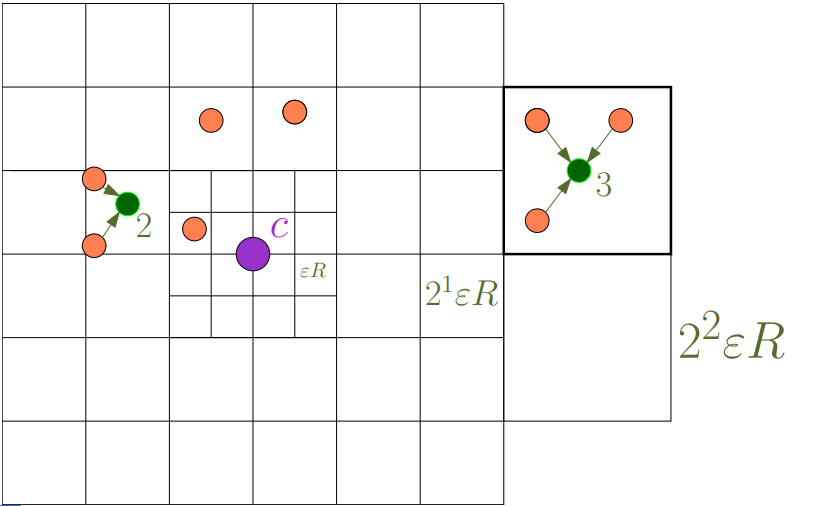
\includegraphics[totalheight=4cm]{grid.png}
    \caption{Krata wykładnicza, gdzie $c = x_{i}$. W najbliższym otoczeniu punktu $c$ widzimy kratę $V_{i,0}$ z długością komórki równej $r_{0} = \epsilon R$.
    Dla uproszczenia pomijam zmienne w mianowniku wcześniej podanej definicji $r_{j}$.
    Kolejny poziom to krata $V_{i,1}$ o długości komórek równej $r_{1} = 2 \epsilon R$.
    Zielone punkty to reprezentanci danej komórki, którym przyjmujemy odpowienie wagi równe ilości punktów w komórce. 
    }
\end{figure}

\section{Heurystyka single swap}

W tym podrozdziale opiszemy heurystykę single swap \cite{Arya2004LocalSH}, która jest przykładem techinki \textit{local search}.
Algorytm przedstawi konstrukcję $(25 + \epsilon)$ aproksymacji dla problemu K-means, która zakłada, że na wejściu dostajemy zbiór kandydatów na centra $C$ oraz zbiór $n$ punktów $P \subset \mathbb{R}^d$.
Autorzy powołują się na pracę \cite{Matousek99onapproximate}, którą zastąpimy pracą \cite{10.1145/1007352.1007400} z uwagi na lepsze gwarancje teoretyczne.
Korzystając z podrozdziału 4.2, w którym przedstawiliśmy \cite{10.1145/1007352.1007400}, obliczamy zbiór $C$.
\\~\\
Heurystyka \textit{single swap} działa poprzez wybranie początkowego zestawu $k$ centrów $S$ ze zbioru kandydatów na centra $C$, a następnie wielokrotnej
próbie ulepszenia rozwiązania poprzez usunięcie jednego środka $s \in S$ i zastąpienie go innym centerm $s^{'} \in C - S$.
Niech $S^{'} = S - \{s\} \cup \{s^{'}\}$ będzie nowym zbiorem centrów.
Jeżeli $\phi_{S^{'}}(C_{opt}) \leq \phi_{S}(C_{opt})$ to zastępujemy zbiór $S$ zbiorem $S^{'}$, w przeciwnym przypadku $S$ pozostaje bez zmian.
W praktyce taki proces powtarzamy do momentu, kiedy $|\phi_{S^{'}}(C_{opt}) - \phi_{S}(C_{opt})| < \epsilon$.
Formalnie możemy udowodnić, że dla $\epsilon > 0$, po wielomianiwej liczbie wykonań takiej procedury algorytm zakończy swoje działanie.
Autorzy nie dowodzą tego wprost ale powołują się na pracę \cite{10.1145/380752.380755}.
\\~\\
Dla uproszczenia zakładamy, że algorytm kończy się kiedy pojedyńcza wymiana elementów $s$, $s^{'}$ nie poprawia wyniku.
Taki zbiór centrów nazwiemy \textit{1-stable}.
\begin{definition}
    Zbiór nazywamy \emph{1-stable}, jeżeli:
    \begin{equation}
        \Delta(S - \{s\} \cup \{c\}) \leq \Delta(S)
    \end{equation}
    dla dowolnych $s \in S$ oraz $c \in C_{opt}$.
\end{definition}

\noindent
Dodatkowo wprowadźmy notację:
\begin{equation}
    \Delta(S) = \Delta_{P}(S) = \sum_{q \in P} \Delta(q,s_{q}) = \sum_{q \in P} d(q, s_{q})^{2}
\end{equation}
gdzie $s_{q}$ to najbliższy punkt dla $q$ w $S$ oraz $P \subset \mathbb{R}^{d}$.

\begin{definition}
    Niech $N_{S}(s)$ oznacza sąsiedzctwo punktu $s$, czyli zbiór punktów z $P$, dla których punkt $s$ jest najbliżej spośród punktów z $S$.
\end{definition}

W ramach tego podrozdziału udowodnimy następujące twierdzenie.

\begin{thm}{\cite{10.1145/1007352.1007400}}
    Niech $S$ będzie zbiorem $k$ centrów spełniającym własność 1-stable oraz niech $C_{opt}$ będzie optymalnym zbiorem $k$ centrów.
    Wtedy zachodzi następującą nierówność:
    \begin{equation}
        \Delta(S) \leq 25 \Delta(C_{opt})
    \end{equation} 
\end{thm}

\begin{lemma}{\cite{10.1145/1007352.1007400}}
    Dla danego skończonego podzbioru $S$ punktów z $\mathbb{R}^d$, niech $c$ będzie centroidem dla $S$. Wtedy dla dowolnego $c^{'} \in \mathbb{R}^d$, $\Delta(S, c^{'}) = \Delta(S, c) + |S|\Delta(c, c^{'})$.
\end{lemma}
\begin{proof}
    Z definicji $\Delta(S, c^{'})$ otrzymujemy:
    \begin{equation}
        \Delta(S, c^{'}) = \sum_{u \in S} \Delta(u, c^{'}) =  \sum_{u \in S} (u - c^{'}) (u - c^{'})
    \end{equation}
    \begin{equation}
         = \sum_{u \in S} ((u - c) + (c - c^{'})) ((u - c) + (c - c^{'}))
    \end{equation}
    \begin{equation}
        = \sum_{u \in S} ((u - c)(u - c)) + 2((u - c)(c - c^{'})) + ((c - c^{'})(c - c^{'}))
    \end{equation}
    \begin{equation}
        = \Delta(S, c) + 2\Big( (c - c^{'}) \sum_{u \in S} (u - c) \Big) + |S|((c - c^{'})(c - c^{'}))
    \end{equation}
    \begin{equation}
        = \Delta(S, c) + |S|\Delta(c,c^{'})
    \end{equation}
    Ostanie przejście korzysta z faktu, że jeżeli $c$ jest centroidem $S$ to z definicji zachodzi $\sum_{u \in S} (u - c) = 0$.
\end{proof}

%\epsilon
\noindent
Dla każdego optymalnego $c \in C_{opt}$ wyznaczamy $s_{c}$, czyli najbliższe heurestyczne centrum z $S$ dla $c$.
W takim kontekście powiemy, że $c$ jest \textit{schwytane} przez $s_{c}$.
Tutaj warto zaznaczyć, że każde optymalne centrum jest schwytane przez jedno heurystyczne centrum, ale każde heurystyczne centrum może być schwytane przez kilka optymalnych centrów.
Heurystyczne centrum nazwiemy \textit{samotnym} jeżeli nie jest schwytane przez żadne optymalne centrum.

\begin{proof}
    Dowód twierdzenia zaczniemy od zdefniowania podziału $S$ oraz $C_{opt}$ na zbiory $S_{1}, \dots, S_{r}$ oraz $O_{1}, \dots, O_{r}$ dla pewnego $r$, gdzie $|S_{i}| = |O_{i}|$ dla $i = 1, \dots, r$.
    \\~\\
    Dla każdego heurystycznego centrum $s_{i}$, które schywało jakąś liczbę $m \geq 1$ optymalnych centrów, tworzymy zbior $S_{i}$, który będzie zawierał $s_{i}$ oraz dowolne $m-1$ osamotnionych heurystycznych centrów.
    Analogicznie, zbior $O_{i}$ będzie zawierał wszystkie optymalne centra schwytane przez $s_{i}$.
    Rysunek 4.2 obrazuje tak zdefiniowany podział.
    \\~\\
    \noindent
    Następnie będziemy chcieli zdefiniować \textit{swap pary}.
    Dla każdego podziału $|S_{i}| = |O_{i}| = 1$, tworzymy z nich parę.
    Dla każdego podziału, który zawiera więcej schwytanych centrów, czyli $|S_{i}|, |O_{i}| \geq 1$, tworzymy pary między osamotnionymi heurystycznymi centrami a optymalnymi centrami.
    Każde optymalne centrum jest związane z jednym heurystycznym oraz każde osamotnione centrum jest przyporządkowane co najwyżej dwóm optymalnym centrom.
    Centra łaczymy dowolnie. 
    Rysunek 4.2 przedstawia przykładowe swap pary.
    \begin{figure}[H]
        \centering
        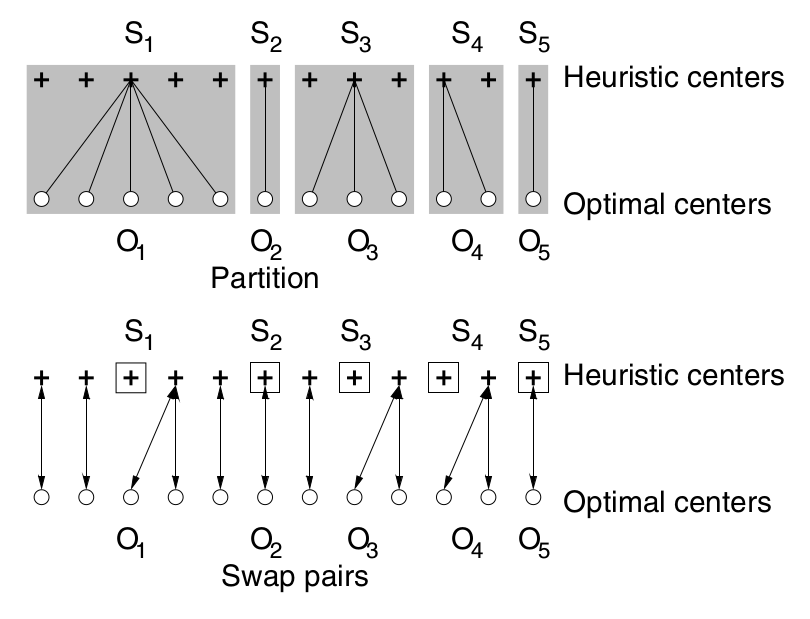
\includegraphics[totalheight=8cm]{swap.png}
        \caption{}
    \end{figure}
    Teraz chcielibyśmy znaleźć ograniczenie górne na zmianię funkcji $\Delta$ po skorzystaniu ze swap pary $(s, o)$.
    Zaczniemy od obliczenia najbliższych centrów z $S - \{s\} \cup \{o\}$ dla punktów z $P$.
    Dla punktów $p \in P$, które należą do $N_{O}(o)$ zmiana $\Delta$ będzie następująca:
    \begin{equation}
        \sum_{q \in N_{O}(o)} (\Delta(q, o) - \Delta(q, s_{q}))
    \end{equation}
    Każde $q \in N_{S}(s) \setminus N_{O}(o)$ straciło przypisane mu centrum $s$ zatem punkt $q$ musi otrzymać nowe centrum.
    Niech $o_{q}$ będzie oznaczało najbliższe centrum dla punktu $q$.
    Skoro $q \notin N_{O}(o)$ to $o_{q} \neq o$, zatem $s$ nie schwytało $o_{q}$.
    A więc po skorzystaniu ze swap pary, $s_{o_{q}}$, najbliższe heurystyczne centrum dla $o_{q}$ nadal istnieje.
    Zmiana $\Delta$ po wyborze nowych centrów jest co najwyżej równa:
    \begin{equation}
        \sum_{q \in N_{S}(s_{i}) \setminus N_{O}(o_{i})} (\Delta(q, s_{o_{q}}) - \Delta(q, s))
    \end{equation}
    Na tym etapie dowodu koniecznie będzie wprowadzenie dwóch lematów.
    
    \begin{lemma}{\cite{10.1145/1007352.1007400}}
        Niech $S$ będzie zbiorem $k$ centrów spełniającym własność 1-stable oraz niech $C_{opt}$ będzie optymalnym zbiorem $k$ centrów.
        Wtedy zachodzi następującą nierówność:
        \begin{equation}
            0 \leq \Delta(O) - 3\Delta(S) + 2R
        \end{equation}
        gdzie, $R = \sum_{q \in P} \Delta(q, s_{o_{q}})$.
    \end{lemma}
    \begin{proof}
        Ponieważ $S$ jest 1-stable to:
        \begin{equation}
           0 \leq \Delta(S) -  \Delta(S - \{s\} \cup \{o\})
        \end{equation}
        \begin{equation}
            = \sum_{q \in N_{O}(o)} (\Delta(q, o) - \Delta(q, s_{q})) + \sum_{q \in N_{S}(s) \setminus N_{O}(o)} (\Delta(q, s_{o_{q}}) - \Delta(q, s))
        \end{equation}
        Aby rozszerzyć sumę na wszystkie możliwe swap pary zauważamy, że dla każdego optymalnego centrum, jest ono swapnięte tylko raz.
        Zatem każdy punkt $q$ kontrybuuje w pierwszej sumie tylko raz.
        Po drugie zaważmy, że różnca w drugiej sumie jest zawsze niezerowa dlatego rozszerzając zakres sumowania mozemy tylko zwiększyć sumaryczny wynik.
        \begin{equation}
            0 \leq \sum_{q \in P} (\Delta(q, o_{q}) - \Delta(q, s_{q})) + \sum_{q \in P} (\Delta(q, s_{o_{q}}) - \Delta(q, s_{q}))
        \end{equation}
        \begin{equation}
            0 \leq \sum_{q \in P} \Delta(q, o_{q}) - 3 \sum_{q \in P} \Delta(q, s_{q}) + 2\sum_{q \in P} \Delta(q, s_{o_{q}})
        \end{equation}
        \begin{equation}
            0 \leq \Delta(C_{opt}) - 3 \Delta(S) + 2R
        \end{equation}
    \end{proof}
    \noindent
    Wcześniej zdefiniowane $R$ nazywamy sumarycznym kosztem przepisania centrów.
    Korzystając z lematu 3 przekształcamy:
    \begin{equation}
        R = \sum_{o \in O} \sum_{q \in N_{O}(o)} \Delta(q, s_{o}) = \sum_{o \in O} \Delta(N_{O}(o), s_{o}) 
    \end{equation}
    \begin{equation}
        = \sum_{o \in O} (\Delta(N_{O}(o), o) + |N_{o}(O)| \Delta(o, s_{o})
    \end{equation}
    \begin{equation}
        = \sum_{o \in O} \sum_{q \in N_{O}(o)} (\Delta(q, o) + \Delta(o, s_{o}))
    \end{equation}
    \begin{equation}
        \leq \sum_{o \in O} \sum_{q \in N_{O}(o)} (\Delta(q, o) + \Delta(o, s_{q}))
    \end{equation}
    \begin{equation}
        = \sum_{q \in P} (\Delta(q, o_{q}) + \Delta(o_{q}, s_{q}))
    \end{equation}
    gdzie ostatnia nierówność bazuje na fakcie, że dla każdego $q \in N_{O}(o)$ mamy $\Delta(o, s_{o}) \leq \Delta(o, s_{q})$.
    Następnie korzystamy z nierówności trójkąta.
    \begin{equation}
        R \leq  \sum_{q \in P} \Delta(q, o_{q}) + \sum_{q \in P} ( d(o_{q}, q) + d(q, s_{q}))^{2}
    \end{equation}
    \begin{equation}
        = \sum_{q \in P} \Delta(q, o_{q}) + \sum_{q \in P} ( d(o_{q}, q)^{2} + 2d(o_{q}, q)d(q, s_{q}) + d(q, s_{q})^{2})
    \end{equation}
    \begin{equation}
        = 2\sum_{q \in P} \Delta(q, o_{q}) + \sum_{q \in P} \Delta(q, s_{q}) + 2\sum_{q \in P} d(o_{q}, q)d(q, s_{q})
    \end{equation}
    \begin{equation}
        = 2\Delta(O) + \Delta(S) + 2\sum_{q \in P} d(o_{q}, q)d(q, s_{q})
    \end{equation}
    \begin{lemma}{\cite{10.1145/1007352.1007400}}
        Niech $\langle o_{i} \rangle$ oraz $\langle s_{i} \rangle$ będą ciągami liczb rzeczywistych, dla których zachodzi:
        \begin{equation}
            \alpha^2 = \frac{\sum_{i} s_{i}^{2}}{\sum_{i} o_{i}^{2}}
        \end{equation}
        dla pewnego $\alpha > 0$.
        Wtedy:
        \begin{equation}
            \sum_{i=1}^{n} o_{i} s_{i} \leq \frac{1}{\alpha} \sum_{i=1}^{n} s_{i}^{2}
        \end{equation}
    \end{lemma}
    \begin{proof}
        Z nierówności Schwarza:
        \begin{equation}
            \sum_{i=1}^{n} o_{i} s_{i} \leq \Big( \sum_{i=1}^{n} o_{i}^{2} \Big)^{\frac{1}{2}} \Big( \sum_{i=1}^{n} s_{i}^{2} \Big)^{\frac{1}{2}}
        \end{equation}
        \begin{equation}
            = \Big( \frac{1}{\alpha^{2}}\sum_{i=1}^{n} s_{i}^{2} \Big)^{\frac{1}{2}} \Big( \sum_{i=1}^{n} s_{i}^{2} \Big)^{\frac{1}{2}}
        \end{equation}
        \begin{equation}
            = \frac{1}{\alpha} \sum_{i=1}^{n} s_{i}^{2}
        \end{equation}
    \end{proof}
    Niech $o_{i}$ będzie ciągiem $d(q, o_{q})$ oraz niech $s_{i}$ będzie ciągiem $d(q,s_{q})$ dla wszystkich $q \in P$.
    Z tego wynika, że błąd aproksymacji możemy przedstawić jako:
    \begin{equation}
        \alpha^{2} = \frac{\Delta(S)}{\Delta(O)} = \frac{\sum_{q \in P} d(q,s_{q})^{2}}{\sum_{q \in P} d(q,o_{q})^{2}} =\frac{\sum_{i=1}^{n} s_{i}^{2}}{\sum_{i=1}^{n} o_{i}^{2}}
    \end{equation}
    Korzystając z lematu 5:
    \begin{equation}
        R \leq 2\Delta(O) + \Delta(S) + 2\sum_{q \in P} d(o_{q}, q)d(q, s_{q}) 
    \end{equation}
    \begin{equation}
        \leq 2\Delta(O) + \Delta(S) + \frac{2}{\alpha}\sum_{q \in P} d(q, s_{q})^{2} 
    \end{equation}
    \begin{equation}
        = 2\Delta(O) + \Delta(S) + \frac{2}{\alpha}\Delta(S)
    \end{equation}
    \begin{equation}
        = 2\Delta(O) + \Big(1 + \frac{2}{\alpha} \Big)\Delta(S)
    \end{equation}
    Z lematu 4 wiemy, że:
    \begin{equation}
        0 \leq \Delta(O) - 3\Delta(S) + 2R
    \end{equation}
    \begin{equation}
        = \Delta(O) - 3\Delta(S) + 2\Big(2\Delta(O) + \Big(1 + \frac{2}{\alpha} \Big)\Delta(S)\Big)
    \end{equation}
    \begin{equation}
        \leq 5\Delta(O) - \Big(1 - \frac{4}{\alpha} \Big)\Delta(S)
    \end{equation}
    Powyższą nierówności możemy przekształcić do postaci:
    \begin{equation}
        \frac{5}{1-\frac{4}{\alpha}} \geq \frac{\Delta(S)}{\Delta(O)} = \alpha^{2}
    \end{equation}
    \begin{equation}
        5 \geq \alpha^{2} \Big(1 - \frac{4}{\alpha} \Big)
    \end{equation}
    \begin{equation}
        0 \geq (\alpha - 5)(\alpha + 1)
    \end{equation}
    To implikuje, że $\alpha \leq 5$, więc wcześniej zdefiniowany błąd aproksymacji możemy ograniczyć przez $\alpha^{2} \leq 25$, co kończy dowód twierdzenia 4.2.
\end{proof}
\section{Podsumowanie}

W tej części przedstawimy algorytm budowania coresetu z \cite{DBLP:journals/ki/MunteanuS18}.
Na początku obliczmy $10$-aproksymację dla problemu K-means korzystając z pracy \cite{Arya2004LocalSH}.
W części 4.3 opisaliśmy konstrukcję, której użyjemy w implementacji.
Ma ona trochę większy błąd aproksymacji ale jak sami autorzy \cite{DBLP:journals/ki/MunteanuS18} stwierdzają w swojej pracy, nie ma to dużego znaczenia w kontekście całości.
Dowolna aproksymacja o stałym błedzie może zostać użyta w tej metodzie.
Na potrzeby analizy zakładamy, że obliczamy $10$-aproksymację $C^{'}$ oraz dany na wejściu zbiór punktów $A \subset \mathbb{R}^d$ należy do przestrzeni Euklidesowej.
\\~\\
Geometryczna dekompozycja bazuje na dyskretyzacji punktów z $A$, czyli na zgrupowaniu ze sobą najbliższych punktów, a następnie zbudowaniu ważonego zbioru punktów $S$ o zredukowanym rozmaiarze.
Taką techinkę mogliśmy już zobaczyć w części 4.2, gdzie odpowiednio grupowaliśmy punkty w komórki kraty wykładniczej.
\\~\\
Praca \cite{DBLP:journals/ki/MunteanuS18} przedstawia inną technikę, która bazuje na budowaniu kul o wykładniczo rosnącym promieniu wokół każdego punktu z $C^{'}$.
Będziemy znaczynać od promieni równych $\frac{1}{n}OPT$ a kończyć na $10 OPT$, gdzie $OPT = \phi_{opt}^{k}(A)$.
Dla takich kul będziemy budować $\epsilon$-pokrycie kuli.

\begin{lemma}{\cite{pisier_1989}}
    Niech $U$ będzie sferą jednostkową w $d$-wymiarowej przestrzeni euklidesowej.
    Wtedy dla $0 < \epsilon < 1$, istnieje \textit{$\epsilon$-pokrycie} $B$ o rozmiarze $\Big(1 +\frac{2}{\epsilon}\Big)^{d}$, czyli dla każdego punktu $p \in U$ zachodzi:
    \begin{equation}
        \min_{b \in B} ||p-b|| \leq \epsilon
    \end{equation}
\end{lemma}

\noindent
Niestety ale nie istnieją efektywne metody budowania takich $\epsilon$-pokryć.
My w analizie przyjmujemy, że  $|B| = \epsilon^{-O(d)}$.
Jako referenrencję jak zbudować taką konstrukcję autorzy sugureują analizę pracy \cite{chazelle_2000}.
Jest to problematyczne w kontekście implementacji jednak tą kwestię poruszymy w następnym rodziale.
\begin{lemma}{\cite{DBLP:journals/ki/MunteanuS18}}
    Niech $a$, $b$, $c$ będą punktami z przestrzeni euklidesowej.
    Wtedy dla dowolnego $\epsilon \in (0,1)$ zachodzi:
    \begin{equation}
        \Big| ||a-c||^{2} - ||b-c||^{2} \Big| \leq \frac{12}{\epsilon} ||a-b||^2 + 2\epsilon||a-c||^2
    \end{equation}
\end{lemma}
\begin{lemma}
    Niech $A$ będzie zbiorem $n$ punktów z $\mathbb{R}^d$, $B^{i}$ będzie kulą o promieniu $r_{i} = \frac{2^{i}}{n}\sum_{x \in A} ||x||^{2}$ oraz niech $S^{i}$ będzie $\frac{\epsilon}{3}$-pokryciem kuli $B^{i}$.
    Zdefinujemy $S = \bigcup_{i=0}^{\log 10n} S^{i}$. 
    Wtedy:
    \begin{equation}
        \sum_{x\in A} \min_{s \in S} ||x - s||^{2} \leq \epsilon^{2} \sum_{x \in A} ||x||^{2}
    \end{equation}
\end{lemma}
\begin{proof}
    Niech $A_{close}$ będzie zbiorem punktów z kwadrtem normy euklidesowej równej co najwyżej $\frac{1}{n}\sum_{x \in A}||x||^{2}$ oraz niech $A_{far}$ będzie zbiorem pozostałych punktów.
    Ponieważ $|A_{close}| \leq n$, to:
    \begin{equation}
        \sum_{x\in A_{close}} \min_{s \in S^{0}} ||x - s||^{2} \leq |A_{close}|\frac{1}{n}\frac{\epsilon^{2}}{9}\sum_{x \in A_{close}}||x||^{2} \leq \frac{\epsilon^{2}}{9}\sum_{x \in A_{close}}||x||^{2}
    \end{equation}
    \noindent
    Dla punktów ze zbioru $A_{far}$, rozpatrzmy punkt $x \in B^{i} \setminus B^{i-1}$ dla $i \in \{1, ..., \log10n \}$.
    Zatem:
    \begin{equation}
       \min_{s \in S^{i}} ||x - s||^{2} \leq \frac{\epsilon^{2}}{9} r_{i}^{2} \leq \frac{4\epsilon^{2}}{9} r_{i-1}^{2} \leq \frac{4\epsilon^{2}}{9} ||x||^2
    \end{equation}
    Sumując po wszystkich punktach otrzymujemy:
    \begin{equation}
        \sum_{x\in A} \min_{s \in S} ||x - s||^{2} \leq \frac{\epsilon^{2}}{9}\sum_{x \in A_{close}}||x||^{2} + \frac{4\epsilon^{2}}{9} \sum_{x \in A_{far}}||x||^2 < \epsilon^{2} \sum_{x \in A} ||x||^{2}
    \end{equation}
\end{proof}
\noindent
Taką analizę możemy zaaplikować do każdego punktu z $C^{'}$.

\begin{thm}
    Dla dowolnego zbioru $n$ punktów $A \subset \mathbb{R}^d$ z przestrzeni euklidesowej, istnieje coreset dla problemu k-means zawierający $O(k\epsilon^{-d} \log n)$ punktów, gdzie $d$ to wymiar (skończny) przestrzeni.
\end{thm}
\begin{proof}
    Dla każdego z $k$ center ze zbioru $C^{'}$ mamy $\log 10n$ kul o rożnych promieniach.
    Dla każdej takiej kuli o promieniu $r$ obliczamy $\frac{\epsilon}{16}r$-pokrycie oraz dla każdego punktu $x \in A$, niech $B(x)$ będzie najbliższym punktem w sumie wszystkich pokryć kul.
    Z lematu 8 wynika, że:
    \begin{equation}
        \sum_{x\in A} ||x - B(x)||^{2} \leq \Big( \frac{\epsilon}{16} \Big)^{2} \cdot 10 \cdot OPT
    \end{equation}
    Teraz, rozpatrzmy dowolny zbiór $k$ center $C$:
    \begin{equation}
        \sum_{x\in A} \min_{c \in C} ||x - c||^{2} - \sum_{x\in A} \min_{c \in C} ||B(x) - c||^{2}
    \end{equation}
    \begin{equation}
        \leq_{\text{lemat 7}} \frac{12}{\epsilon} \sum_{x\in A} ||x - B(x)||^{2} + 2\epsilon \sum_{x\in A} \min_{c \in C} ||x - c||^{2}
    \end{equation}
    \begin{equation}
        \leq \frac{12}{\epsilon} \Big( \frac{\epsilon}{16} \Big)^{2} \cdot 10 \cdot OPT + 2\epsilon \sum_{x\in A} \min_{c \in C} ||x - c||^{2}
    \end{equation}
    \begin{equation}
        \leq 2\epsilon \cdot OPT + 2\epsilon \sum_{x\in A} \min_{c \in C} ||x - c||^{2}
    \end{equation}
    \begin{equation}
        \leq 4\epsilon \sum_{x\in A} \min_{c \in C} ||x - c||^{2}
    \end{equation}
    gdzie ostatnia nierówność zachodzi ponieważ $OPT \leq \sum_{x\in A} \min_{c \in C} ||x - c||^{2}$ dla dowolnego zbioru center $C$.
    \\~\\
    Skalując $\epsilon$ przez $\frac{1}{4}$ kończymy dowód.
    Rozmiar coresetu to $O(k\epsilon^{-d} \log n)$, ponieważ obliczamy $k \log 10n$ razy $(\frac{\epsilon}{64})$- pokrycie o rozmiarze $\epsilon^{-O(d)}$.
\end{proof}


\chapter{Podsumowanie}\label{analysis}

W ramach naszej pracy przygotowaliśmy implementację opisanych konstrukcji budowania coresetów dla problemu $k$-means.
Całość dostępna jest w repozytorium \url{https://github.com/piotrhm/coreset}, które jest podzielone następująco:
\dirtree{%
.1 algorithm.
.2 geometric.
.3 coreset.py.
.2 lightweight.
.3 coreset.py.
.1 dataset.
.2 s-set.
}
\noindent
Zacznijmy od opisu implementcji konstrukcji przedstawionej w rozdziale 4, czyli geometrycznej dekompozycji.
Wprowadzona w tym rozdziale konstrukcja jest wynikiem czysto teoretycznym, co implikuje kilka problemów implementacyjnych.
\begin{enumerate}
    \item Nie umiemy w szybki sposób obliczać najbliższego sąsiada z danego zbioru dla zbioru punktu.
    Używanie naiwnego podejścia o złożoności $O(n^2d)$ w praktyce, nawet dla niewielkich zbiorów o $n=15000$ skutkuje zauważalnym czasem obliczeń.
    Problem jest szczególnie widoczny w implementacji heurystyki \textit{single swap}, gdzie przy każdej iteracji algorytmu musimy obliczyć funkcję $\phi$ dla nowego zbioru kandydatów na rozwiązanie.
    Częściowym rozwiązaniem tego problemu było użycie biblioteki \textit{sklearn.neighbors} \url{https://scikit-learn.org/stable/modules/neighbors.html}.
    \item Nie umiemy obliczać $\epsilon$-pokryć kul.
    Jest to bardzo bolesne ponieważ nie istnieje rozsądny zamiennik tego rozwiązania.
    W związku tym jedyną alternatywą jest użycie jakieś heurystyki, która w praktyce daje akceptowalne wyniki.
\end{enumerate}

\noindent
Implementacja geometrycznej dekompozycji problemu $k$-means ma następujący schemat:
\begin{enumerate}
    \item Oblicz wielomianową aproksymację problemu $k$-means:
    \begin{enumerate}
        \item Oblicz 2-aproksymację dla problemu $k^{*}$-center korzystając z algorytmu Gonzaleza opisanego w 4.1, gdzie $k^{*} = O(k \log^2 n)$.
        \item Obliczoną 2-aproksymację dla problemu $k^{*}$-center zamień na 20 - aproksymację dla problemu $k^{**}$-means, korzystając z konstrukcji opisanej w 4.2.1, gdzie $k^{**} = O(k \log^3 n)$.
        \item Korzystajac z konstrukcji kraty wykładniczej opisanej w 4.2.3 zamień 20-aproksymację dla problemu $k^{**}$-means na $(\epsilon, k^{**})$-coreset.
        \item Oblicz 25-aproksymację dla problemu $k$-means korzystając z heurystyki single swap, gdzie obliczony $(\epsilon, k^{**})$-coreset jest zbiorem kandydatów na centra.
        \end{enumerate}
    \item Oblicz $\epsilon$-pokrycie dla kul o środkach należących do zbioru $C$, gdzie $C$ to obliczona 25-aproksymacja dla problemu $k$-means.
\end{enumerate}

\noindent
W ogólności, większość algorytmów budowy coresetów bazujach na geometrycznym podejściu cechuje skomplikowana konstrukcja oraz mało atrakcyjna złożoność.
Nasza konstrukcja nie jest w tej kwestii wyjątkiem, jednak tym co ją wyrożnia to kroki 1.(a)-1.(c) wyżej opisanego schematu.
Autorzy pracy \cite{10.1145/1007352.1007400} zauważyli, że dla odpowiednio dużego $k$ jesteśmy w stanie szybko obliczać najbliższego sąsiada z danego zbioru dla punktu \cite{Arya2004LocalSH}.
Jest to kluczowe w kontekście analizy gwarancji teoretycznych jednak w praktyce zaproponowne rozwiązania są zupełnie nieużyteczne.
Kolejną optymalizacją jest zainicjalizowanie początkowego rozwiązania $S$ w heurystyce single swap korzystając z algorytmu Gonzaleza.
Pomysłodawcami są autorzy \cite{10.1145/1007352.1007400}, którzy nie dowodzą w żaden sposób faktycznej poprawy jakości wyników czy czasu działania.
\\~\\
Zaimplementowana przez nas konstrukcja geometrycznej dekompozycji problemu $k$-means miała być próbą zaproponowania konkurencyjnego rozwiązania dla lightweight coresetu.
Niestety ale z uwagi na wyżej opisane problemy nie udało się dostarczyć rozwiązania, które byłoby zgodne z udowodnionymi gwarancjami teoretycznymi.
Aktualny stan implementacji przedstawia mocną bazę do dalszych optymalizacji.   
\\~\\
Naturalnym pytaniem jest to czy istnieje \textit{praktyczny} i \textit{łatwy} w implementacji algorytm budujący coreset dla problemu $k$-means.
Podobne pytanie zadali sobie autorzy pracy \cite{bachem2017scalable}, którzy zaproponowali konstrukcję o nazwie lightweight coreset.
Zauważyli, że większość dostępnych algorytmów jest bardzo skomlikowana w implementacji albo nie daje żadnych gwarancji teoretycznych.
Całą konstrukcję można streścić w kilku linijach kodu widocznego poniżej.
\\
\lstset{language=Python}
\begin{lstlisting}
    def _compute_coreset(self):
        #Algorithm 1 Lightweight coreset construction
        dist = np.power(self.X-self.X.mean(axis=0), 2).sum(axis=1)
        q = 0.5/self.X.shape[0] + 0.5*dist/dist.sum()
        indices = np.random.choice(self.X.shape[0], size=self.m, replace=True)
        X_cs = self.X[indices, :]
        w_cs = 1.0/(self.m*q[indices])
        return X_cs, w_cs
\end{lstlisting}
\nocite{*}
\bibliographystyle{acm}
\bibliography{bibliography}
\tableofcontents
\end{document}
